\documentclass{standalone}
\usepackage{tikz}
\usetikzlibrary{arrows}
\usetikzlibrary{shapes.multipart}
\usetikzlibrary{shapes,snakes}
\usepackage[bitstream-charter]{mathdesign}

\begin{document}
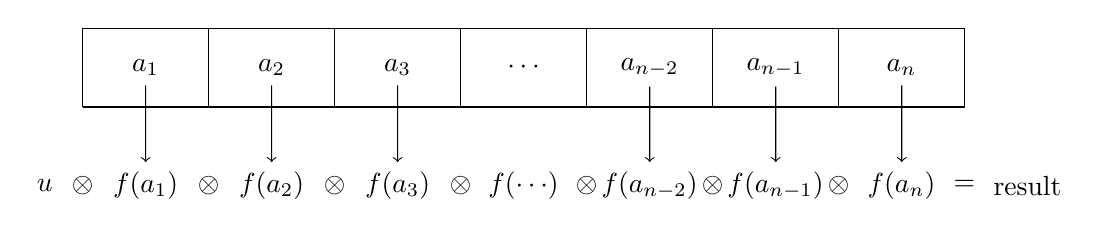
\begin{tikzpicture}[xscale=1.6]
    \draw (0,0) grid (7,-1);
    \foreach \x/\t/\k in {.5/$a_1$/0,1.5/$a_2$/1,2.5/$a_3$/2,3.5/$\cdots$/3,4.5/$a_{n-2}$/4,5.5/$a_{n-1}$/5,6.5/$a_n$/6} {
        \node (a\k) at (\x,-0.5) {\t};
        \node (f\k) at (\x,-2) {$f($\t$)$};
    }
    \foreach \k in {0,1,2}
      \draw[->] (a\k) -- (f\k);
    \foreach \k in {4,5,6}
      \draw[->] (a\k) -- (f\k);

    \foreach \x in {0,1,2,3,4,5,6}
      \node at (\x,-2) {$\otimes$};

    \node at (7,-2) {$=$}; 
    \node at (7.5,-2) {result};
    \node at (-0.3,-2) {$u$};
\end{tikzpicture}
\end{document}

